\documentclass[twocolumn]{jarticle}%,2pt
\setlength{\columnsep}{3zw} 

\title{\vspace{5mm}\large{あああああああ}\vspace{-15mm}}
%\title{\tiny{}}
\date{}


\usepackage{textcomp}
\usepackage[sc]{mathpazo}
\usepackage[scaled]{helvet}
\usepackage{amsmath,amssymb}
%\usepackage{otf}%字体が変更できる
\usepackage{color}
\usepackage{threeparttable}
\usepackage[dvipdfmx,hiresbb]{graphicx}%
\usepackage{float}
\usepackage{fancyhdr}
\usepackage{titlesec}
\usepackage[top=30truemm,bottom=30truemm,left=20truemm,right=20truemm]{geometry}

%define for header%\titleformat*{\section}{\large\bfseries}
\titleformat*{\section}{\large\bfseries}
\renewcommand{\ttdefault}

%Header
\pagestyle{fancy}%ページ番号を入れるか決めてるっぽい.
\rhead{}
\lhead{出願区分 : 情報科学区分 \\ 氏名 : 小黒司友 \\ 現在の専門 : 情報工学 \\ 希望希望研究室: インタラクティブメディア設計学研究室}

\begin{document}
\normalsize
%\author %
\maketitle

\section{はじめに}
\thispagestyle{fancy}

私が,奈良先端科学技術大学院大学(以下NAIST)で取り組みたい研究テーマは「ああああああああああ」である.本稿では,\ref{current}章でこれまでの修学内容について,\ref{want}章で貴学で取り組みたい研究テーマの研究背景及び目的・先行研究・提案手法について述べ,結びとする.

\section{現在行っている研究}\label{current}
私が現在行っている研究を以下に述べる.

これまでに,歩行者集団の移動の円滑性・効率性に着目する交通流シミュレータが開発されていた.しかし,歩行者と空間を共有するパーソナルモビリティやロボットを,安全かつ快適に運用するには,個々の歩行者の振る舞いや歩行者間の相互作用までシミュレートする必要がある.

そこで本研究では,歩行者に近い歩行ルール(歩行モデル)を持つアバターを扱うシミュレータを作成することを最終的な目標とする.

図\ref{fig:environment}に示すようなシミュレーション空間中でシミュレーションを行う.また,被験者がシミュレーション中にどのような行動を行うのかをデータとして得るために,アバターのうちの一体としてアバターを操作し,シミュレーションに参加することができるモード(アバター操作モード) を用いる.被験者は,図\ref{fig:user_view}のような一人称視点で他のアバターの様子を観察しながら操作を行う.

歩行モデルとアバター操作モードを用いてシミュレーションを行った結果から,歩行モデルの評価を行う.歩行モデルの評価は,効率性,安定性,安全性,みための自然さの観点から行う.

\begin{figure}[H]
    \begin{tabular}{cc}
      %---- 最初の図 ---------------------------
      \begin{minipage}[t]{0.45\hsize}
        \centering
        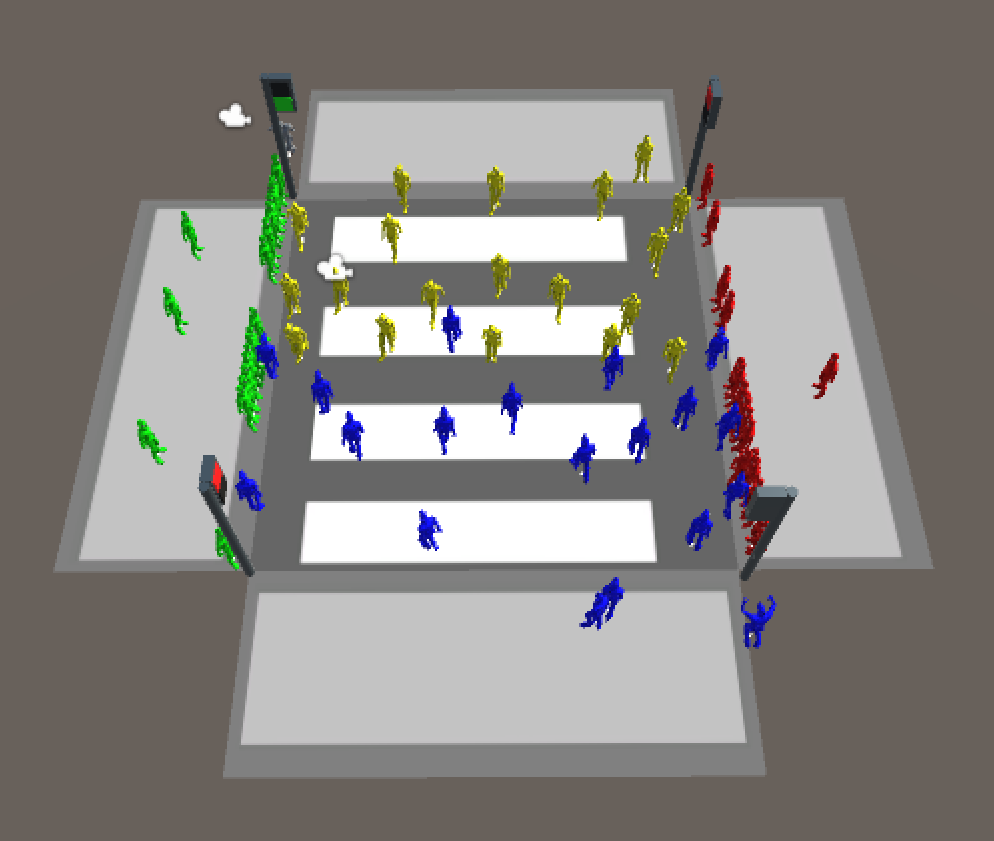
\includegraphics[keepaspectratio, scale=0.11]{images/environment.JPG}
        \caption{シミュレーション環境}
        \label{fig:environment}
      \end{minipage} &
      %---- 2番目の図 --------------------------
      \begin{minipage}[t]{0.45\hsize}
        \centering
        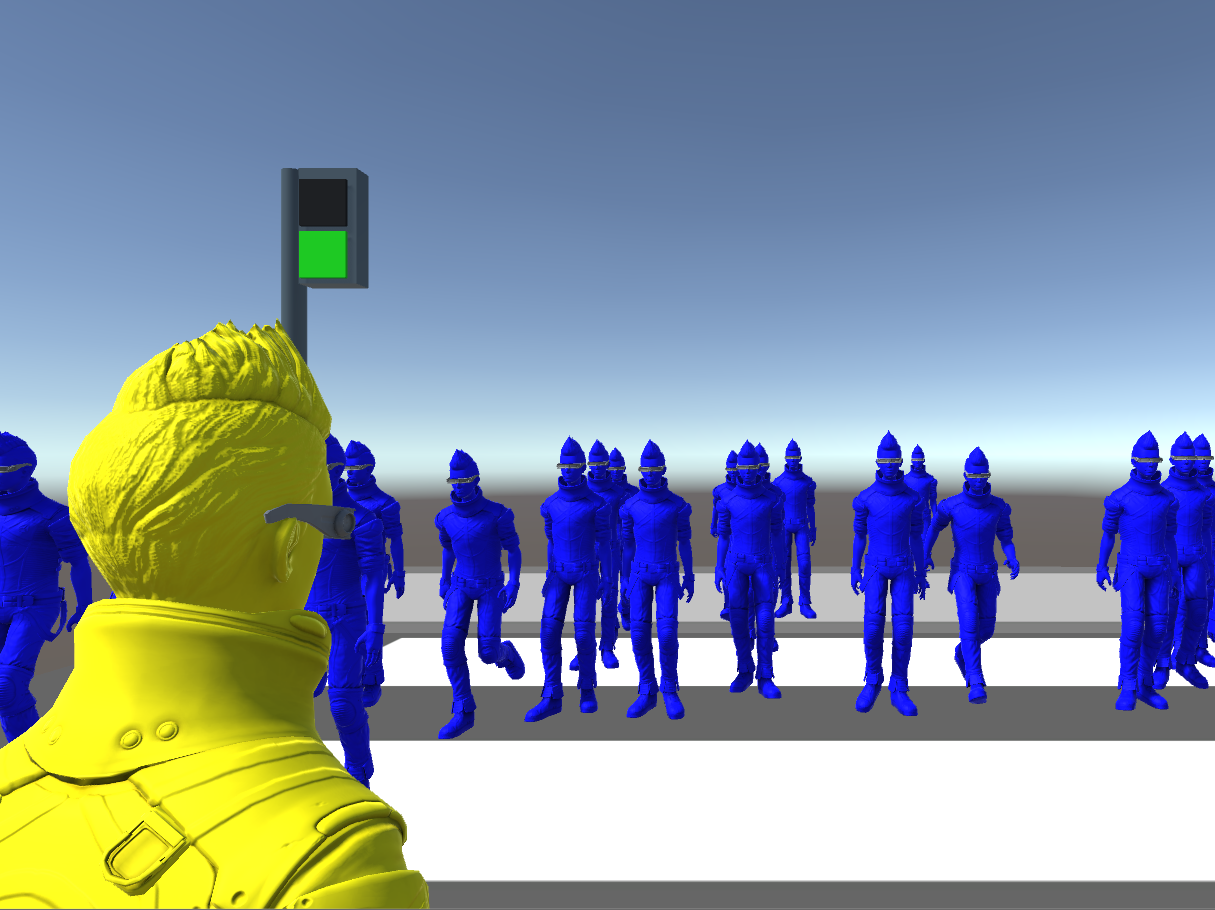
\includegraphics[keepaspectratio, scale=0.1]{images/user_view_mini.JPG}
        \caption{被験者が体験するシミュレーションの様子}
        \label{fig:user_view}
      \end{minipage}
      %---- 図はここまで ----------------------
    \end{tabular}
  \end{figure}

\section{貴学において取り組みたい研究}\label{want}

\section{おわりに}

\bibliographystyle{jplain}
\bibliography{Untitled}

\end{document}
